\documentclass[conference]{IEEEtran}
\IEEEoverridecommandlockouts
% The preceding line is only needed to identify funding in the first footnote. If that is unneeded, please comment it out.
\usepackage{cite}
\usepackage{amsmath,amssymb,amsfonts}
\usepackage{algorithm,algpseudocode}
\usepackage{graphicx}
\usepackage{textcomp}
\usepackage{xcolor}
\usepackage{graphicx}
\usepackage{listings}
\usepackage{booktabs}
\graphicspath{ {./} }
\def\BibTeX{{\rm B\kern-.05em{\sc i\kern-.025em b}\kern-.08em
    T\kern-.1667em\lower.7ex\hbox{E}\kern-.125emX}}
\begin{document}

\title{Parallelized Distributed Storage System\\
}

\author{\IEEEauthorblockN{1\textsuperscript{st} Arjun Pherwani}
\IEEEauthorblockA{\textit{PM, Programmer} \\
\textit{UCF CS Dept.}\\
Orlando, USA \\
arjunp@knights.ucf.edu}
\and
\IEEEauthorblockN{2\textsuperscript{nd} Cameron Cuff}
\IEEEauthorblockA{\textit{Programmer} \\
\textit{UCF CS Dept.}\\
Orlando, USA \\
ctcuff@knights.ucf.edu}
\and
\IEEEauthorblockN{2\textsuperscript{nd} Joseph Giordano}
\IEEEauthorblockA{\textit{Programmer} \\
\textit{UCF CS Dept.}\\
Orlando, USA \\
joseph.giordano@knights.ucf.edu}
\and
\IEEEauthorblockN{2\textsuperscript{nd} Dylan Skelly}
\IEEEauthorblockA{\textit{Programmer} \\
\textit{UCF CS Dept.}\\
Orlando, USA \\
dskelly@knights.ucf.edu}
}
\maketitle

\begin{abstract}
This document is the implementation details and design of the distributed storage system worked on by our team.
\end{abstract}

\begin{IEEEkeywords}
distributed storage, encryption, parallelization
\end{IEEEkeywords}

\section{Introduction}

\subsection{The Problem}
When thinking of storage we often think of it in unbroken files and folders.
All files that are associated with each other are stored next to each other in folders.
This methodology works quite well for humans because this is how we stored information
prior to the advent of computing, however,
this methodology breaks when we try to extend it to the cloud.

To give the reader an example, let's take a hypothetical storage provider, Storage Corp.
This company has some existing storage infrastructure which is the servers they have running on premises.
For simplicity sake lets say their infrastructure is limited to 2 drives each being 1 TB in size.

Now, they have 3 large files to store. Each file is 600 GB in size.
Since the three files will collectively be 1.8 TB in space and we have 2 TB of total space,
on the surface this is easy to solve.
Let's try to do that right now. The first file is 600 GB, and goes to the first drives.
Since 1 TB is greater than 600 GB we can easily store that and have room to spare.
400 GB of room to be precise.

\begin{figure}[h]
\caption{Two drives that still have capacity but cannot be used in the traditional way.}
\centering
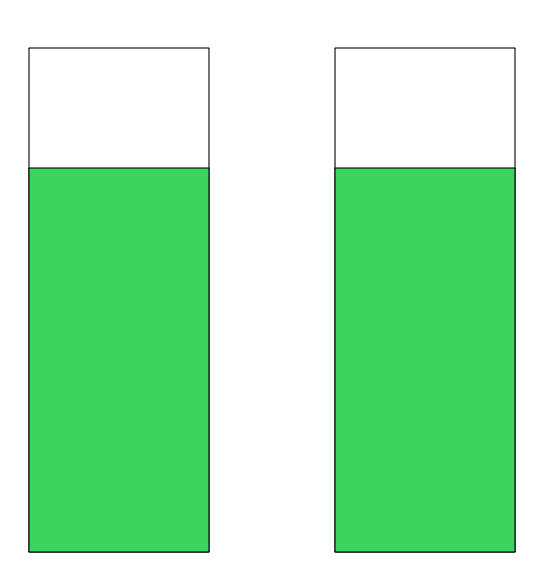
\includegraphics[width=0.25\textwidth]{database.png}
\end{figure}

Now onto the second large file. This file is 600 GB large also, but the first drive only has 400 GB of capacity.
No problem, we can store that in the second disk.
This disk has ample space.
After storing the second file, we now have 400 GB of capacity each in our two drives.
This sums up to 800 GB which is more than enough to store a 600 GB large file.
However there is a slight hiccup.
We don't have enough space in each of the drives to individually hold the third file (as shown in Fig. 1).

\subsection{The Solution}
We plan to solve this problem for our project.
Now to be clear, this is a solved problem.
It's quite easy to solve in fact.
Storage Corp should just take the large file, break it into smaller chunks and store those.
This way there is no wasted space.
Our project was inspired by MongoDB's GridFS system.
What they do is break larger files into smaller chunks which are easy to store and then just assemble those at runtime later and return the complete file to the user.

While this is great, we wanted to explore this problem ourselves.
For one, because we couldn't find the source code to GridFS around we figured what they did must be a proprietary solution that we cannot see.
Because we were interested in the mechanics of how they made this work we decided to come up with our own solution from scratch to do this.
Below are the implementation details of our solution.

\section{Implementation}

At the most basic level our project will be a command line tool.
The idea is that the user points it in the direction of a file (for the scope of this project we are restricting the file type to .txt)
and the tool breaks the file apart into different chunks, encrypts those chunks and stores them in an s3 bucket.
In doing so, it creates a record of the location of the chunks, how to decrypt those chunks and the order in which the chunks should be placed to access them.

Of course, this by itself is not parallel or multithreaded in any way whatsoever.
Neither is the above paragraph detail enough to really explain what we are doing so in the below subsections we will be going into more detail on that.

\subsection{Chunking}

The process of "chunking" involves reading a file into memory and splitting it into smaller
pieces that are easier to manage. The size of each chunk is determined by the user. As an example,
if we define a chunks size $C$ (such that $C \in \mathbb{N}$), a file that is $N$ bytes will
be split into $\lfloor \frac{N}{C} \rfloor$ chunks. It should be noted that the last chunk
may be significantly smaller than the others if $\frac{N}{C}$ yields a noticeable remainder.

\medskip
\indent
Because each chunk is encrypted (a topic mentioned in a later section), every chunk isn't
guaranteed to be exactly of size $C$. This is due to the fact that the encryption method
used is not a one-to-one character mapping. Encrypting one singe character may instead
yield two characters.

\medskip
\indent
After the encryption step, each chunk is uploaded to an AWS bucket. Chunks are given a random
name generated with a UUID library. Each chunk is prefixed with the order in which it was split.
This makes it easier to piece chunks back together in a later process. As a final step, a JSON
file is saved to user's computer that contains instructions on hho to piece together each encrypted
chunk. This JSON file (aptly named \textit{keystore.json}) holds the master encryption key along
with the nonce keys used to encrypt each chunk.

\medskip
\indent
The benefit of file chunking is the potential space saved from breaking the file into pieces.
If an application uses multiple databases and one database has a small amount of storage
available, a file that exceeds that limit won't be able to fit in that space. However, we'd
now have unused and potentially wasted space. When we take a large file and split it into many
smaller pieces, we can utilize this space across many databases.

\subsection{Encryption / Decryption}

As mentioned in an earlier section, each file chunk is encrypted with the ChaCha20-Poly1305
cipher. ChaCha20-Poly1305 is an AEAD (Authenticated Encryption with Additional Data) cipher
that combines the ChaCha20 stream cipher with the Poly1305 message authentication code.

\medskip
\indent
ChaCha20 is a stream cipher that takes a secret key and some sort of nonce value (a value
that cannot be used more than once for the same key) and generates a stream of deterministic
random bits called the \textit{keystream}. The primary purpose of the keystream is to XOR
it with plaintext to produce ciphertext. Because the plaintext doesn't need to be known
in advance to generate the stream, this approach allows the ChaCha20 algorithm to be
very efficient and easily parallelizable. Additionally, this works fell when implemented
with file splitting. This means that smaller blocks of text can be encrypted in parallel
because the ChaCha20 cipher doesn't need to know what it's encrypting.

\medskip
\indent
Published in 2004, Poly1305 is a cryptographic message authentication code (MAC) that can be
used with and encrypted or unencrypted message to generate a keyed authentication token. This
token is used to guarantee the integrity and validity of a given message. Poly1305 is
extremely high speed and can take advantage of additional hardware to reduce latency for
long message. Similar to ChaCha20, this means Poly1305 can easily be parallelizable.

\medskip
\indent The general process for file encryption is as follows:
\begin{enumerate}
    \item
        Generate a master encryption key using a UUID generation function. This master key
        must be 32 bytes.
    \item
        For every file chunk, generate a random nonce key using a UUID generation function.
        This nonce key must be 24 bytes and, along with the master encryption key, will
        be used to encrypt this chunk using the ChaCha20-Poly1305 algorithm.
	\item 
		Create a JSON file (named \textit{keystore.json}) that contains the encryption
		key and nonce keys used to encrypt each file chunk.
\end{enumerate}

\medskip
\indent The general process for file encryption is as follows:
\begin{enumerate}
	\item Load the keystore JSON file into memory and read the master encryption key
	\item
		Take each file chunk and sort them alphanumerically from 0 to $N$, where
		$N$ is the total number of chunks.
	\item
		For every encrypted file chunk, use the master encryption key and associated
		nonce key to decrypt the file chunk into a plain text string.
	\item
		Once all chunks have been decrypted, combine each decrypted string into one
		large string to form the original plaintext.
\end{enumerate}

\subsection{Parallelization}

We have identified potential tasks that we can hand off to other threads which would parallelize the code.
It goes without saying that the more work that can be done in parallel the faster our code will run.
Rust has great support for concurrency and we hope to leverage this to achieve the maximum speedup possible.
x
Because of the nature of the project, theoretically, once a chunk has been created everything about it can be handed off to a thread to take care of.
This can go right from encryption, to sending the item off to the bucket.
On this flip side, during the retrieval process, we can potentially parallelize the retrieval from the S3 bucket all the way to decryption.
At the moment, our code is completely sequential and we are working on parallelizing the aforementioned tasks.

The parallelized storage and retrieval algorithm is described below.

\begin{algorithm}
	\caption{Parallelized Bucket Storage}\label{storage}
	\begin{algpsuedocode}
		% \ForAll{$i$ \in Threads}
		% \State BucketWrite{$i$}
		% \Return{Response}
	\Procedure{BucketWrite}{$i$}
	\State $c\gets Creds$
	\If{$b$.empty()}
	\State $b\gets Bucket$
	\Else
	\State $Threads[$i$] \gets b$
	\EndElse
	\EndProcedure
	\end{algpsuedocode}
\end{algorithm}

% create cipher and keystore
% chunk the file into small chunks
% parallel iterate (map and collect):
%   encrypt chunks
%   create random filename for chunk
%   return (encryption_scheme, filename, encrypted_bytes)
% create filenames with the chunk index
% for each encrypted chunk:
%   create an async function to write this chunk to aws bucket
%   create a futures stream with a buffer for the functions
%   execute each function

\begin{algorithm}
	\caption{Parallelized Encryption \& Bucket Storage}\label{storage}
	\begin{algpsuedocode}
	\Procedure{chunkFile}{$file$}
	\Return $chunks$
	\EndProcedure
	\Procedure{write}{$file$}
	\State $ciph\gets Cipher$
	\State $keystore\gets [...]$
	\State $chunks\gets$ chunkFile($file$)
	\end{algpsuedocode}
\end{algorithm}

\subsection{Storage and Retrieval}

In order to simulate the experience of storing and retrieving from a file store we decided to use AWS S3 buckets.
There are a couple of reasons for this, the first and most important being that this project was intended to be an
into how a file can be split apart into smaller and more manageable fragments (chunks) and how we could parallelize that.
By that logic it didn't seem worth it to try to figure out a complicated way of storing it.

On the other hand we also wanted something that was non-trivial.
By this we mean that we did not want to just paste the files in local storage. 

For those reasons we decided we wanted to go with some cloud storage option.
But there were still other options like Azure Blob Storage.
Unfortunately we could not use blob storage because it does not have an officially supported Rust SDK.
S3 on the other hand seemed to have promising support which is why we picked AWS S3 buckets. Additionally, S3 allows for
large PUT operations, all the way up to 5GB, making it capable of testing sizeable file inputs, and storing up to 50TB in 
one S3 instance. Another benefit is the ability to pay as we go, with assurance that large tests will not be interrupted 
even in during significant spikes in network traffic. The reliability and availability of S3 storage makes it a perfect 
platform for facilitating our storage system and developing to scale. 

The rust-s3 library simplifies interactions with Amazon S3 buckets with built in asynchronous API features, 
which can be deactivated if needed. Full suppport for operations including put, get, and delete allows for 
cleaner Rust code. In terms of file security, the methods presign\_get and presign\_put allows us to upload files
to a bucket, and selectively distribute the link to team members without concern for files being visible as
they are stored at a presigned URL. 

One of the rust-s3 library's default features is Tokio. The Tokio asynchronous runtime for Rust provides flexible, 
thread-safe, and performant APIs for storing and retrieving objects in our buckets. GET and PUT functions for objects
and object streams with Tokio methods are tokio::io::AsyncWriteExt and tokio::io::AsyncReadExt. The Tokio runtime harnesses
a work-stealing scheduler, a multithreaded scheduler in which a processor has an assigned thread queue with their own 
sequential instructions. However, what distinguishes the work-stealing scheduler is the fact that threads can spawn new tasks 
that can be parallelized with the code currently being executed. As the new tasks are placed on the processor's queue. When the 
queue is empty, a processor examines other queues in an effort to adopt extra tasks, effectively dealing with idle processors 
by balancing the excess workload spawned by other threads. This is where the strategy gets its name, by \textit{stealing} and
distributing work until it is all dealt with by highly parallelized task execution. This can be particularly useful in our 
application, as chunking for multiple files may imply uneven workloads by forking more or less threads across different processors, 
especially when working with larger files, or scaling the application in the future.

Figure 2 displays the work-stealing concept with an example for two processors possessing multiple threads and a queue of CPU-bound 
tasks that are to be balanced on the available processes. In the example, we observe that the second process, P2, is currently running less
operations, so it has the ability to steal tasks from the threads of the first process, P1. The motivation for work-stealing is to
limit the amount of work for a single process, and distribute the load amongst the available processesors in the form of threads. 

\begin{figure}[h]
	\caption{Work-stealing method as a means to load balance several tasks.}
	\centering
	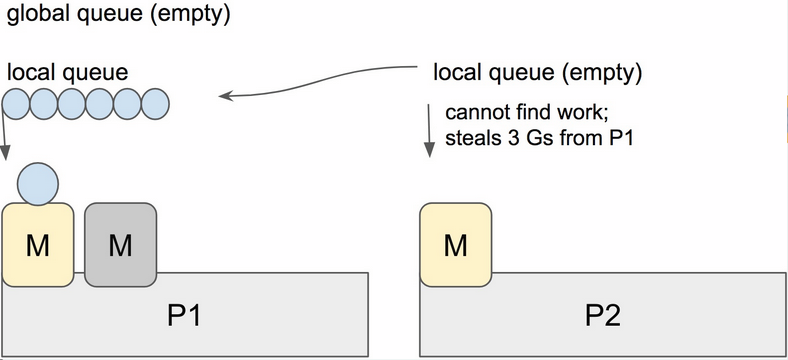
\includegraphics[width=0.45\textwidth]{work-stealing.png}
\end{figure}

The futures library was used to accomodate parallel uploading of encrypted chunks to our s3 bucket. The futures library is a
Rust crate with abstractions for asynchronous computing, of which, we employ the StreamExt trait.

Futures are conceptually equivalent to the Promise objects used in other 
languages, which signifies the awaited response from an asynchronous function call, which may currently be unknown when the Promise
is instantiated. As such, Futures will indicate the outcome of an asynchronous operation (success or failure). In our code, the StreamExt 
trait and enclosed .iter() function is used to execute each function corresponding to a bucket write operation for the s3 upload of each 
encrypted chunk.


\subsection{Why Rust?}

We picked Rust primarily because we all wanted learn it and now seemed like a great time to try it out.
On a language level Rust has an excellent dependency management solution, Cargo.
Another thing we like about Rust is that it's strongly typed but it infers the types from assignment.
Finally, we wanted our code to be as performant as possible.

All that being said because Rust does a lot of unique things with it's concept of ownership we constantly
find ourselves wrestling with the language to get any work done.
Tools like IntelliSense and TabNine do help speed up our development time.

In addition to development benefits, Rust provides optimal runtime performance compared to other languages,
especially for concurrent applications. Community opinion is split on the issue of concurrency for different
programming languages and runtimes. Typically, Go and Rust are considered to have the greatest performance,
while languages such as JavaScript coupled with popular runtimes such as Deno are easier to develop in. Between
Go and Rust, Rust is found to have more consistency benefits [10]. Although the p\_threads library used with C-based
languages demonstrate higher performance, they do not include the guardrails that Rust requires when building
multithreaded programs which catch likely errors and prevent development overhead [9]. For these reasons, Rust theoretically 
provides the optimal environment for evaluating concurrent performance in applications, even though faster methods do 
exist. The decision to use Rust is a combination of performance and development considerations.

\subsection{Testing}

We believe that to write code of high quality testing is a requirement.
This is why we are in the process of writing tests for our code.
While this isn't a requirement and neither is it a priority for us we still believe we should do it and are doing it.

\section{Results}
We compare runtimes for sequential and parallel execution of chunk encryption and uploading for files of variable size.
All files were encrypted with chunk size of 255,000 bytes. Results are divided between tests where uploading to the s3 bucket 
was and was not performed, since the larger number of asynchronous, IO-bound operations presents an unpredictable confound 
which may amplify or diminish the differences observed between sequential and parallel runtimes. 
The Tokio runtime and Futures runtime both facilitate upload operations, whereas the Rayon runtime is used for most CPU-bound 
tasks. In summary, we compare performance for the encryption alone (without AWS uploads) against encryption and uploading together, 
with the understanding
that it may reveal which operations are benefitting more of less from parallelization. Of course, we cannot run upload operations
without first encrypting due to the architecture of our solution, so those results are not attainable nor particularly relevant.

\begin{table}[ht]
\centering
\caption{Without AWS Uploading}
\begin{tabular}[t]{lccc}
\toprule
File Size&Sequential&Parallel&\% Improvement\\
\midrule
71.4 MB&212 ms&67 ms&68.396\%\\
3.34 GB&9,598 ms&5,345 ms&44.311\%\\
10.49 GB&30,583 ms&21,100 ms&31.007\%\\
\bottomrule
\end{tabular}
\end{table}%

\begin{table}[ht]
	\centering
	\caption{With AWS Uploading}
	\begin{tabular}[t]{lccc}
	\toprule
	File Size&Sequential&Parallel&\% Improvement\\
	\midrule
	71.4 MB&265,212 ms&8437 ms&96.819\%\\
	3.34 GB&N/A&292,658 ms&N/A\\
	\bottomrule
	\end{tabular}
\end{table}%

\subsection{Without AWS uploading}
Figure 3 shows a line graph displaying runtime performance versus file size for the sequential and parallel encryption
algorithms.

\begin{figure}[h]
	\caption{Sequential and parallel encryption for variable file size inputs.}
	\centering
	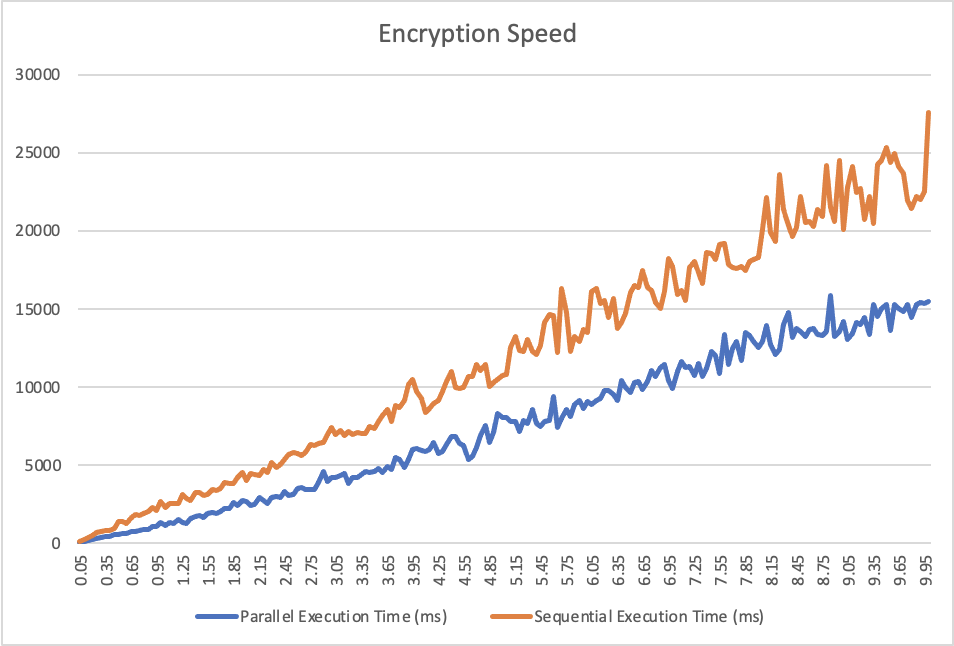
\includegraphics[width=0.45\textwidth]{encryption-speed-line.png}
\end{figure}

Figure 5 shows the performance improvement by \% difference in milliseconds.

\begin{figure}[h]
	\caption{Runtime improvement of parallel over sequential execution, along with speedup.}
	\centering
	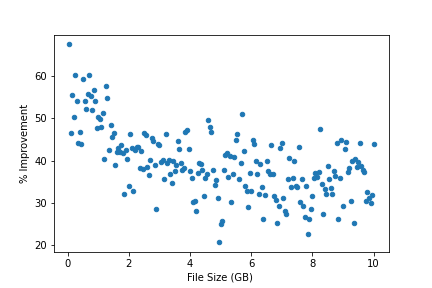
\includegraphics[width=0.50\textwidth]{execution-improvement.png}
	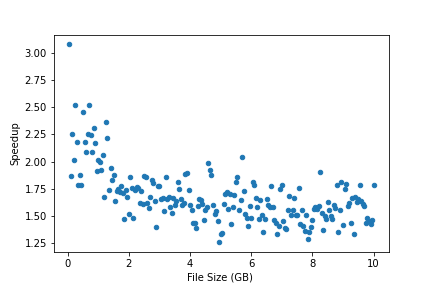
\includegraphics[width=0.50\textwidth]{execution-speedup.png}
\end{figure}

The speedup observed without AWS uploading suggests that the Rayon functions responsible for parallelizing
the CPU-bound tasks alone fails to provide an adequate improvement in runtime when increasing file size. This is 
indicated by the negative slope of the speedup found by dividing the old runtime (sequential) by the new runtime (parallel).
Specifically, we gather that this algorithm doesn't have a linear speedup, and is thus not considered to be scalable [11].

\subsection{With AWS uploading}

\section{Analysis}
There are a number of viable benchmarks used to evaluate the performance of concurrent systems.

\section{Conclusion}
Due to the confounding factors introduced by IO-bound tasks, we did not observe a speedup suggesting optimal 
parallelization that might be conducive to scalability. Instead, we saw that working with file inputs and 
several Rust runtimes creates a bottleneck on the benefits of concurrency, and a better solution or microservice
architecture must be engineered, if this application is to utilize parallelization in Rust.

\section{Appendix}
\subsection{Team Management and Organization}
We are a fairly small team of busy people.
So while the team size makes it easy to organize, the schedules do not.

A notable point is that our team is not using the Agile methodology because
all the members in our team have a strong distaste for it.
Instead we are using a pseudo-waterfall methodology where some of our members get together
for a short period of time and get as much work done as possible.

We believe that this makes our work easier because there is less overhead of having
to maintain the standard Agile artifacts like Kanban boards and have regularly scheduled stand-ups.

We are using GitHub for version control and Discord for communication.

\subsection{Current Progress}

At the moment we are completely done with a sequential version of the command line app.
This means that we can and take a file, break it into several chunks, encrypt those chunks,
write the encryption key and other relevant information to a shared document and send these
an AWS S3 bucket.

Over the next few weeks our efforts are going to be focused on parallelizing the work we have
already done.

In terms of performance evaluation, it would be useful to visualize the number of threads 
versus performance for each task. Comparisons could be drawn between CPU-bound tasks, IO-bound tasks,
and steps involving encryption and file uploads separately. This analysis could be compared with a 
theoretical prediction by Ahmdahl's law, allowing us to evaluate the parallelization limits for each
algorithm employed in the application. Such details are vital to scaling the distributed storage 
system and providing state-of-the-art performance.

\section{Challenges Faced}

Rust has been for the large part the single biggest challenge we have faced.
This is primarily because all of us are new to the language and we constantly find ourselves
wrestling with the language to get any kind of progress.
One of our team members has described the experience as "learning to program all over again".

Another issue we have found is the abundance of out of date documentation.
This is probably because Rust is a very new language and so it's ecosystem is rapidly evolving.

Working with several asynchronous runtimes makes it difficult to analyze the performance of our solution. For instance,
the work stealing implementation built into Tokio will differ slightly from Rayon. Generally, the Rayon library provides
greater support for CPU-bound operations, while Tokio is better for IO-bound tasks. As a result, the runtimes are utilized in a patchwork manner so as to maximize performance with their
respective strengths, depending on the type of computation they await. 

\section{Program Execution}
To run the code on a file, simply \dots

\section*{Acknowledgment}

Thanks to Professor Dechev for allowing us to do this project.
We realize that it is a bit far removed from the usual flavor
of projects submitted for this class.

Thanks also to the Rust community of Discord, StackOverflow
and other mediums for either answering our questions or having
answered other people's questions that were very similar to our own.

A debt of gratitude is also owed to all the developers who contributed
to the open source Rust crates that we used in our project.

% We are very grateful to Arjun for doing absolutely nothing. Cam was amazing. But we can all agree Arjun is awesome.

\begin{thebibliography}{00}
\bibitem{b1} A. Langley, W.-T. Chang, N. Mavrogiannopoulos, J. Strombergson, and S. Josefsson, The ChaCha Stream Cipher for Transport Layer Security, 24-Jan-2014. [Online]. Available: https://tools.ietf.org/id/draft-mavrogiannopoulos-chacha-tls-01.html.
\bibitem{b2} Y. Nir and A. Langley, “ChaCha20 and Poly1305 for IETF Protocols,” Document search and retrieval page, May-2015. [Online]. Available: https://datatracker.ietf.org/doc/html/rfc7539.
\bibitem{b3} https://tokio.rs/.
\bibitem{b4} https://crates.io/crates/rust-s3.
\bibitem{b5} https://aws.amazon.com/s3/faqs/.
\bibitem{b6} https://docs.rs/futures/latest/futures/
\bibitem{b7} https://developer.mozilla.org/en-US/docs/Web/JavaScript/Reference/Global\_Objects/Promise
\bibitem{b8} https://deepu.tech/concurrency-in-modern-languages-rust/
\bibitem{b9} Pfosi, J., Wood, R., &amp; Zhou, H. (n.d.). A Comparison of Concurrency in Rust and C. Github. 
Retrieved from https://ehnree.github.io/documents/papers/rustvsc.pdf 
\bibitem{b10} https://deepu.tech/concurrency-in-modern-languages-final/
\bibitem{b11} Casanova, Henri; Legrand, Arnaud; Robert, Yves (2008). Parallel Algorithms. CRC Press. p. 10.

% \bibitem{b3} I. S. Jacobs and C. P. Bean, ``Fine particles, thin films and exchange anisotropy,'' in Magnetism, vol. III, G. T. Rado and H. Suhl, Eds. New York: Academic, 1963, pp. 271--350.
% \bibitem{b4} K. Elissa, ``Title of paper if known,'' unpublished.
% \bibitem{b5} R. Nicole, ``Title of paper with only first word capitalized,'' J. Name Stand. Abbrev., in press.
% \bibitem{b6} Y. Yorozu, M. Hirano, K. Oka, and Y. Tagawa, ``Electron spectroscopy studies on magneto-optical media and plastic substrate interface,'' IEEE Transl. J. Magn. Japan, vol. 2, pp. 740--741, August 1987 [Digests 9th Annual Conf. Magnetics Japan, p. 301, 1982].
% \bibitem{b7} M. Young, The Technical Writer's Handbook. Mill Valley, CA: University Science, 1989.
\end{thebibliography}
\vspace{12pt}


\end{document}
